\section{Output Compare \& Input Capture}

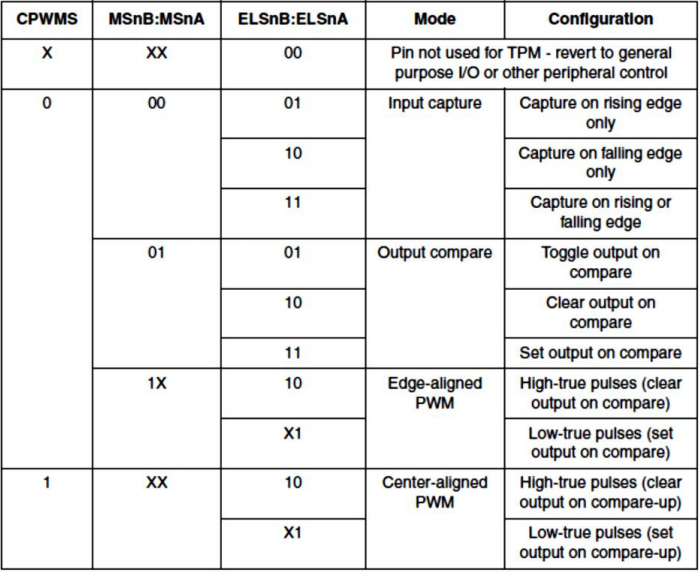
\includegraphics[width=0.5\textwidth]{timer-configuration.png}

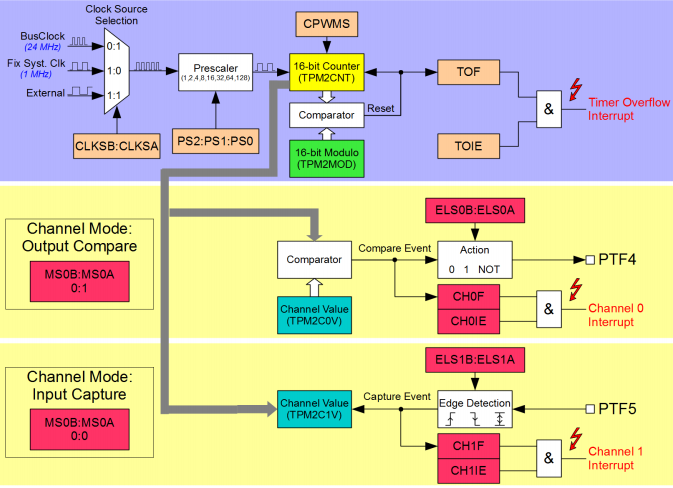
\includegraphics[width=0.5\textwidth]{output-compare-input-capture.png}

\subsection{Timer with Output-Compare}

\textit{
    interrupt is occuring, when the content of the V-Register and
    of the counters have the same value.
}

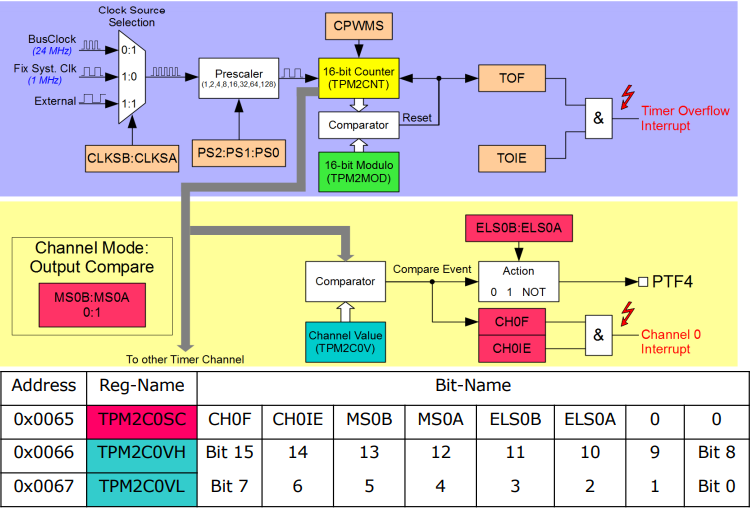
\includegraphics[width=0.5\textwidth]{timer-output-compare.png}

\begin{lstlisting}
void initTimer(void){
    TPM1C1SC_CH1IE = 1; //Channel 1 Timer 1 Interrupt enable
    TPM1C1SC_MS1A = 1; //A=1 ; B=0 - Output Compare
    TPM1C1SC_MS1B = 0;
    TPM1C1SC_ELS1A = 1; //A=1 ; B=0 - Toggle Output on Compare
    TPM1C1SC_ELS1B = 0;
    TPM1C1V = 0x95FF; //set 16bit channel value
    // (is compared with main timer, calc the timer on the base of the clock)
}
interrupt void ISR_outCompare(void){
    TPM1C1SC_CH1F = 0 ; //Timer 1 Channel 1 overflowflag reset
    TPM1C1V += 0x95FF ; //Channel Value is set to new value
    // (add with the value, on how much time needs to pass)
}
\end{lstlisting}

\subsection{Usage Output Compare Mode}

\textit{
    Output Compare is usually used to set / clear or toggle output pins.
    \newline
    The output compare mode can additionally be used to setup
    different timers on base of the same timer wihout
    changing the TPMxMOD value. To use the TPMxCx output pin for other
    purposes, following needs to be set ELSxA:ELSxB=00
}

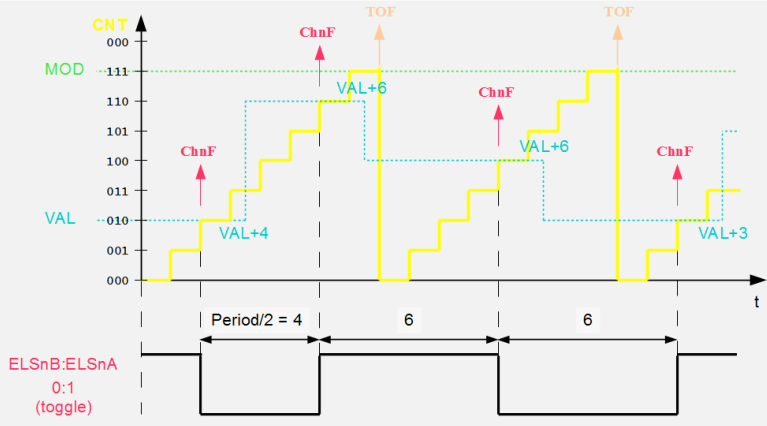
\includegraphics[width=0.5\textwidth]{output-compare-timer-trick.png}

\subsection{Input Capture}

\textit{
    Input capture is used on the timer pins. it enables
    reacting on input (rising/falling or both).\newline
    If an input capture happens, the interrupt is
    executed and the current counter is saved in the channels
    value register for further usage.
}

\subsection{Logic Analyzer}

\textit{
    There are to type of logical analyzers,
    Synchron (zustandsanalyse), Asynchron (Timing Analyse)
}
